\documentclass[11pt]{article}
\usepackage[utf8]{inputenc}
\usepackage[T1]{fontenc}
\usepackage[spanish,es-noshorthands]{babel}
\usepackage[margin=2.5cm]{geometry}
\usepackage{amsmath,amssymb}
\usepackage{graphicx}
\usepackage{booktabs}
\usepackage{xcolor}
\usepackage[colorlinks=true,linkcolor=blue,citecolor=blue]{hyperref}
\usepackage{caption}
\usepackage{parskip}
\usepackage[expansion=false]{microtype}
\sloppy

\title{\textbf{Reconstrucción de logits/corrientes reales\\
y validación de la ecuación de $\beta$ óptimo}}
\author{Walter Quiñonez}
\date{Reporte generado con Claude Code \textperiodcentered\ 6 de septiembre de 2026}

\begin{document}
\maketitle

\begin{quote}\itshape
Se reconstruyen, a partir de los pesos reales guardados
(\texttt{G\_history\_*.npz}) y sin reentrenar nada, los logits/corrientes de
validación de las 18 corridas de \texttt{data\_beta\_grid\_search\_SP/}
(6 INL nominal $\times$ 3 pulsos, $\beta=1$), en función de la época. Se
comparan contra el Monte Carlo sesgado de \texttt{analisis\_beta\_optimo.py}
y contra el Monte Carlo corregido de \texttt{formula\_beta\_optimo\_propuesta/}.
Se prueba la ecuación de Prezioso/LeCun ($\beta_{\text{óptimo}}=\kappa/\sigma_I$,
exponente $-1$ fijo) contra los 18 $\beta$ óptimo experimentales, se
confirma que no la explica, y se re-deriva/confirma una ecuación mejor. Se
cierra con un análisis crítico de si esta ecuación permite reemplazar
\texttt{search\_best\_beta()} por una estimación de un solo paso, o si debe
usarse solo para acotar su rango de búsqueda.
\end{quote}

\tableofcontents

\section{Contexto y objetivo}

Este reporte responde a cuatro pedidos concretos:
\begin{enumerate}
\item Reconstruir, a partir de toda la data de \texttt{data\_beta\_grid\_search\_SP/},
  los logits y corrientes de salida en función de la época.
\item Comparar esa reconstrucción contra el Monte Carlo de
  \texttt{analisis\_beta\_optimo.py}.
\item Analizar la validez de la ecuación de Prezioso sobre la data
  reconstruida, y si no predice bien el $\beta$ óptimo experimental,
  derivar una ecuación mejor.
\item Dar recomendaciones, decir si hace falta más data, y un análisis
  crítico honesto de si es viable estimar $\beta$ óptimo con un método
  tipo Monte Carlo de un solo paso, o si sigue haciendo falta
  \texttt{search\_best\_beta()} (usando la ecuación solo para acotar el
  rango de búsqueda).
\end{enumerate}

\section{Métodos}

\subsection{Reconstrucción exacta de logits/corrientes reales}

\texttt{MemDNN.forward()} es puramente determinista: $I=x\,(G^+-G^-)$, sin
dropout ni ruido (estas 18 corridas tienen ruido=0\%). El \texttt{val\_loader}
usa \texttt{shuffle=False}, y la partición train/val sale de
\texttt{KFold(shuffle=True, random\_state=fold\_seed)} con \texttt{fold\_seed}
guardado en cada \texttt{config\_*.json} --- \texttt{sklearn.KFold} no toca
el estado global de numpy/torch, así que la partición es 100\% reproducible
sin depender de nada más. Estas 18 corridas además guardaron el peso de
\emph{todas} las 100 épocas (\texttt{save\_G\_every=1}).

Con esto: para la corrida $\beta=1$ de cada una de las 18 curvas (carpeta
\texttt{beta\_grid\_search\_SP\_INL\_*}), serie 0, se reconstruye:
\begin{enumerate}
\item la partición de folds (\texttt{KFold} con el \texttt{fold\_seed}
  guardado);
\item los pesos reales de cada fold en cada época
  (\texttt{G\_history\_..\_serie000.npz});
\item el forward pass sobre el set de validación de cada fold, con
  $\beta=1$ (por lo que el logit coincide exactamente con la corriente
  cruda $I$, sin escalar).
\end{enumerate}
\textbf{Sanity check:} la accuracy que sale de este forward reconstruido se
comparó contra la ya guardada en \texttt{resultados\_*.npz} en 2 épocas
$\times$ 5 folds $\times$ 18 curvas = 180 chequeos. Coincide EXACTO
(diferencia $=0$) en el ejemplo detallado
(\texttt{reconstruccion\_logits\_val\_INL\_1e-2\_p\_100\_beta1/}) y se
repitió (1 fold, 2 épocas) para las 18 curvas de este reporte sin ningún
fallo. Script:
\texttt{reconstruccion\_beta\_optimo\_18curvas/reconstruir\_corrientes\_18curvas.py}.

\textbf{Qué NO se reconstruye:} los logits calculados en vivo durante el
propio paso de SGD sobre los minibatches de TRAIN, porque ese shuffle
(\texttt{train\_loader}, \texttt{shuffle=True}) consume el estado global de
\texttt{torch}, fijado una sola vez al arrancar el proceso original y nunca
guardado en ningún archivo. Reproducirlo exigiría re-simular el
entrenamiento completo, no reconstruirlo desde los archivos guardados.

\subsection{Dos Monte Carlo de referencia}

\begin{itemize}
\item \textbf{MC sesgado} (\texttt{analisis\_beta\_optimo.py}, sin
  modificar): pesos combinatorios $w_{ij}=\mathrm{pot}[i]-\mathrm{dep}[j]$
  (en vez de sortear $G^+,G^-$ independientemente del pool combinado, como
  hace la red real) y voltajes de \texttt{np.unique(X\_train)} equipesados
  (en vez de respetar que el 81\% de los píxeles reales son 0). Ya
  documentado en \texttt{analisis\_corrientes\_beta\_optimo/}.
\item \textbf{MC corregido} (\texttt{formula\_beta\_optimo\_propuesta/}):
  pesos vía \texttt{G0\_initialization('random', ...)} real (mismo
  mecanismo que usa la red al inicializarse) y voltajes muestreados
  directamente de píxeles reales de \texttt{X\_train\_mnist.npy}
  (respetando su frecuencia real). Corrige los 2 sesgos de arriba.
\end{itemize}

Ambos se recalculan para las 18 curvas (antes solo existían para 6) en
\texttt{reconstruir\_corrientes\_18curvas.py}.

\subsection{La ecuación de Prezioso}

De \texttt{papers/Reporte\_beta\_optimo\_analitico.pdf} (que a su vez sigue
a Prezioso et al., \emph{Nature} 521, 61, 2015, y LeCun et al.,
\emph{Efficient Backprop}, 1998): modelando $I_i=\sum_{j=1}^N W_{ij}V_j$
como una suma de $N$ términos aprox.\ independientes,
$\mathbb{E}[I]\approx0$ y $\mathrm{Var}[I]=N\,\mathbb{E}[V^2]\,\mathrm{Var}[W]$,
de donde $\sigma_I=\sqrt{N}\,V_{\mathrm{rms}}\,\sigma_W$. Manteniendo
$\mathrm{std}(\beta I)=\beta\sigma_I\sim\kappa=O(1\text{--}10)$ (la
recomendación de LeCun que Prezioso dice haber usado):
\begin{equation}
\beta_{\text{óptimo}} \;\sim\; \frac{\kappa}{\sqrt{N}\,\sigma_W\,V_{\mathrm{rms}}} \;=\; \frac{\kappa}{\sigma_I}
\label{eq:prezioso}
\end{equation}
Esta es la ecuación que se pone a prueba \textbf{literal} (exponente $-1$
fijo, solo se ajusta $\kappa$) en la Sección~4.

\section{Resultado 1: la corriente real converge a un valor casi universal}

\begin{figure}[htbp]
\centering
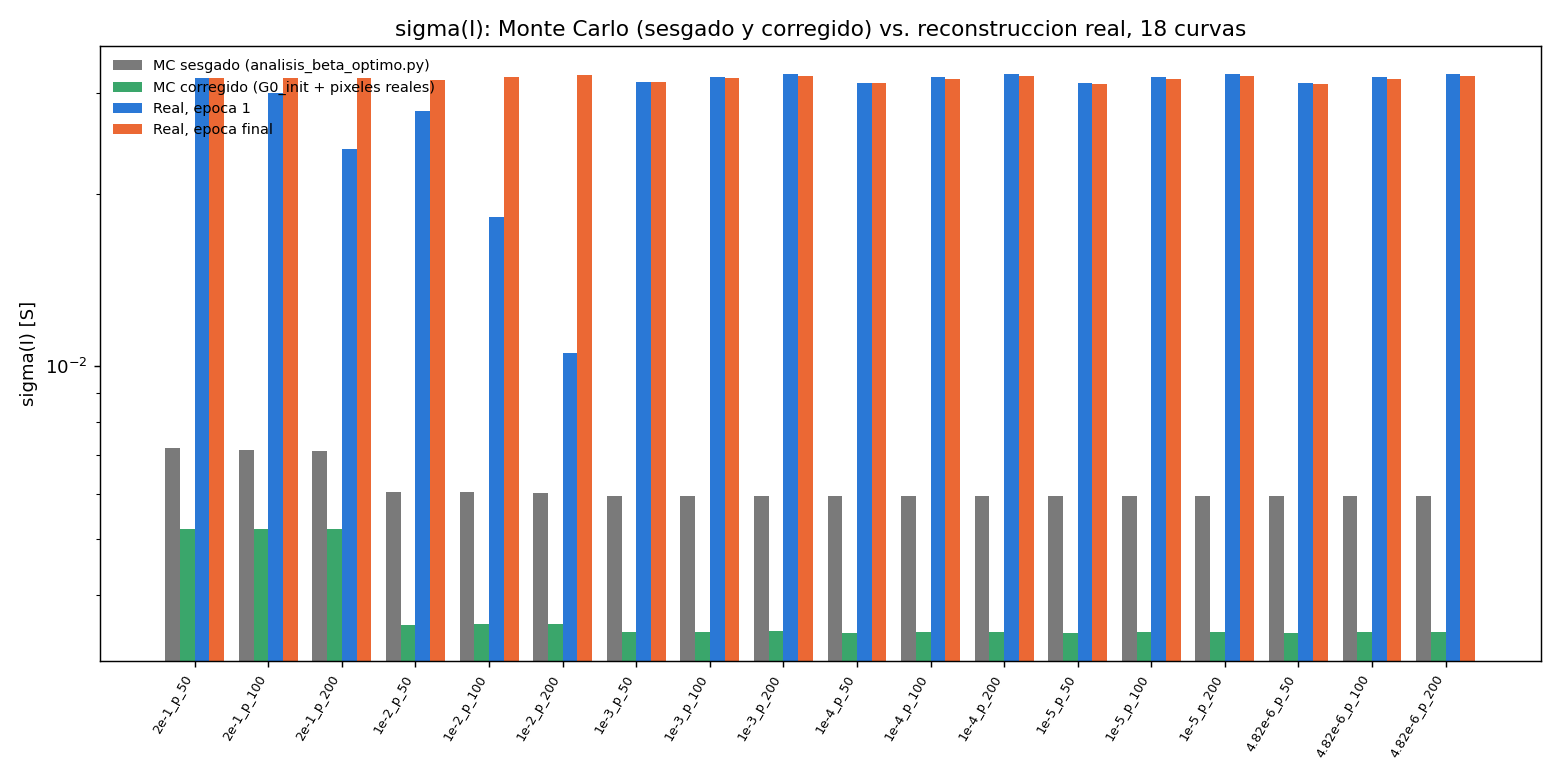
\includegraphics[width=0.85\linewidth]{comparacion_sigma_fuentes.png}
\caption{$\sigma(I)$ por curva: MC sesgado, MC corregido, real época 1, real época final (18 curvas).}
\end{figure}

El hallazgo más llamativo de este reporte: \textbf{$\sigma_I$ real, en la
época final (convergida), es prácticamente la MISMA (0.031--0.032) en las
18 curvas}, sin importar el INL nominal (2e-1 hasta 4.82e-6, casi 4.4
órdenes de magnitud) ni la cantidad de pulsos (50/100/200). Esto es
\textbf{5--9$\times$ más grande} que cualquiera de los dos Monte Carlo
(sesgado: 0.006--0.007; corregido: 0.0034--0.0052).

\begin{figure}[htbp]
\centering
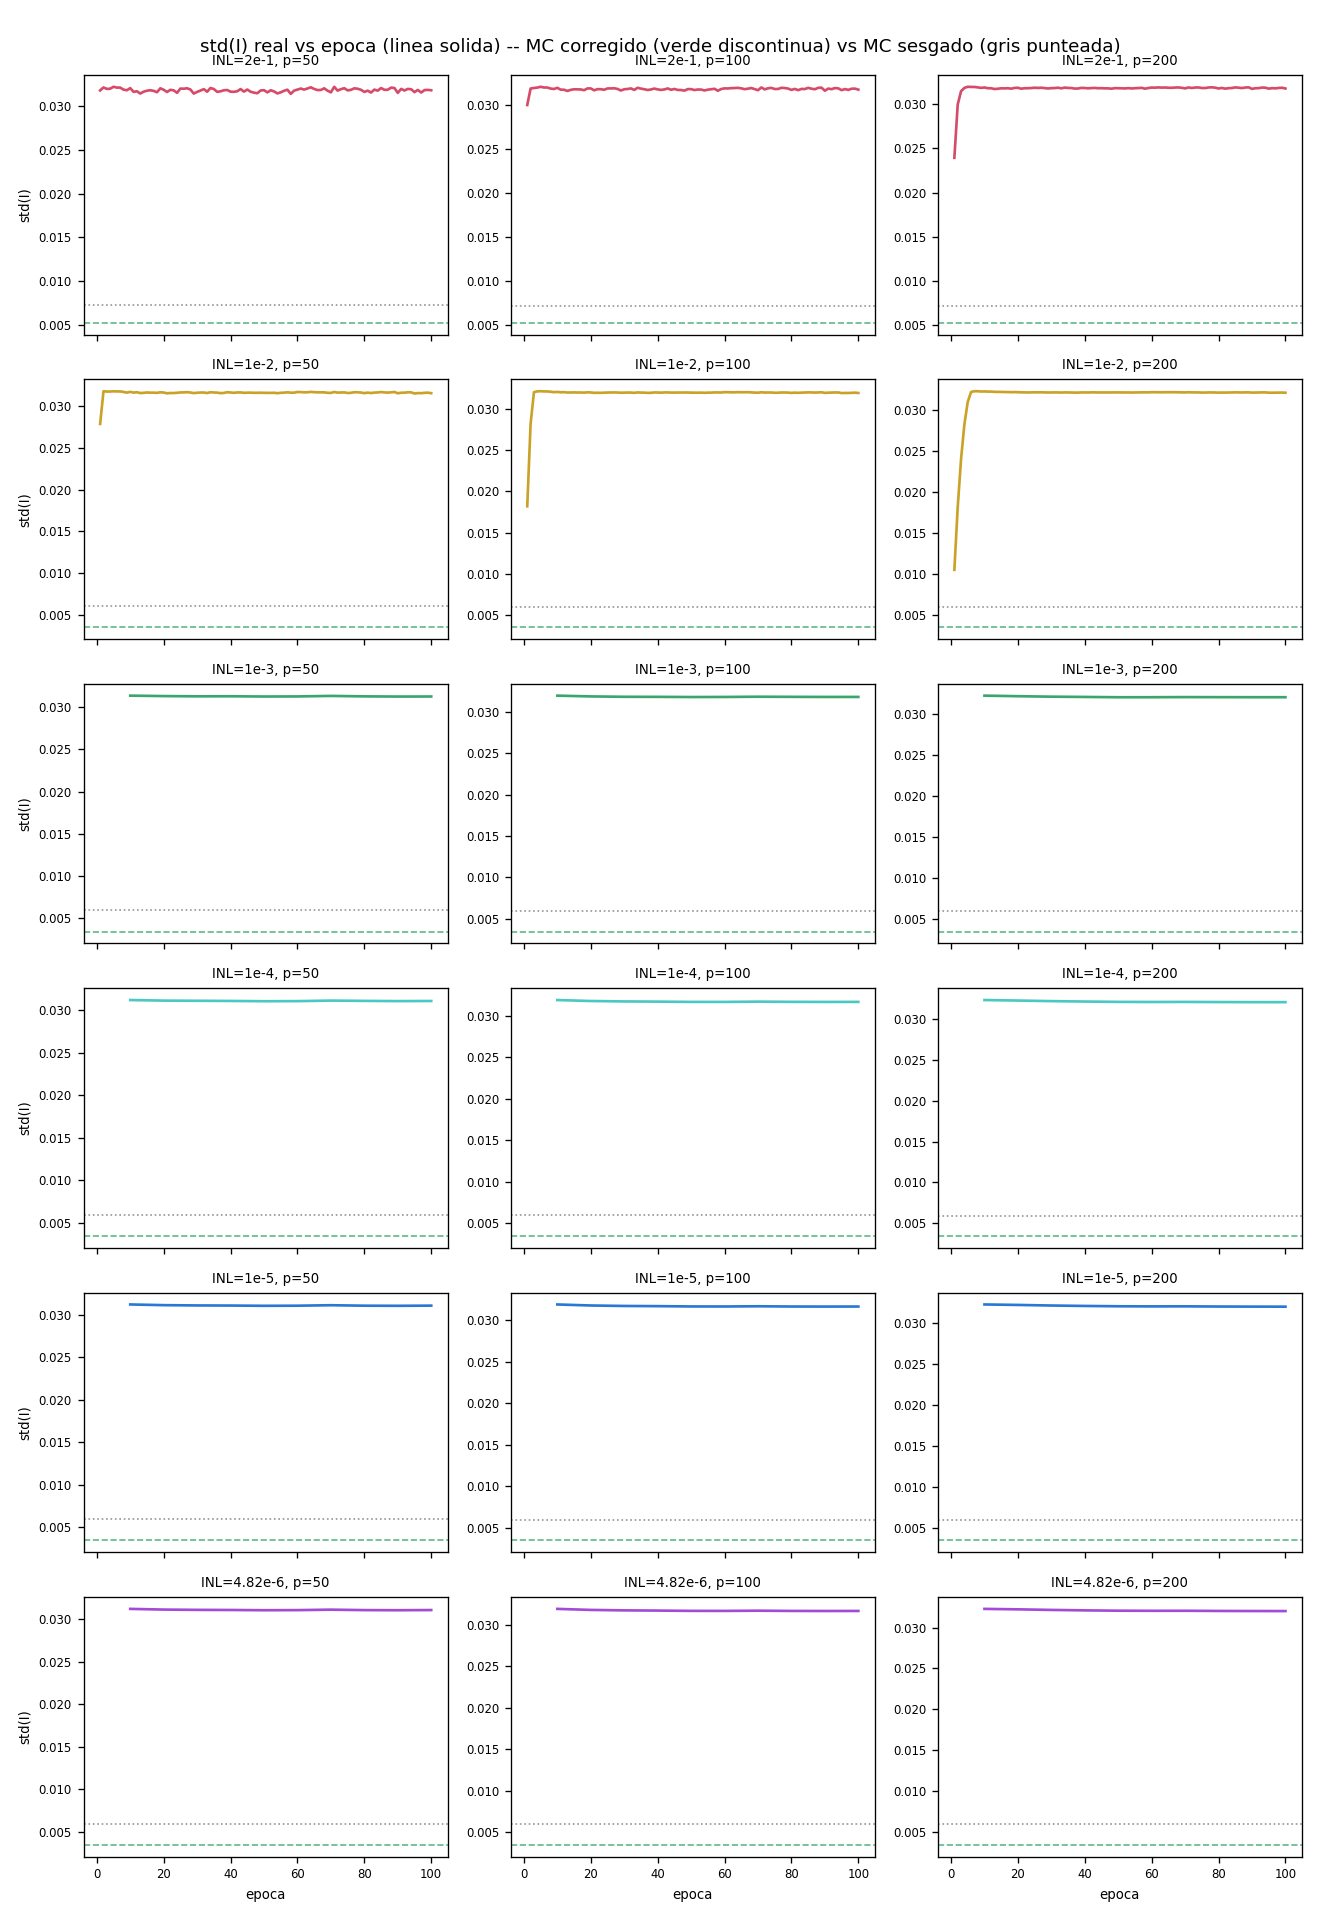
\includegraphics[width=\linewidth]{trayectorias_std_18curvas.png}
\caption{$\mathrm{std}(I)$ real vs.\ época, 18 curvas (líneas de referencia: MC corregido en verde, MC sesgado en gris).}
\end{figure}

Además, esa convergencia es \textbf{casi instantánea}: en la mayoría de las
curvas, $\sigma_I$ ya alcanzó su valor final (o algo muy cercano) desde la
\'epoca 1--5, y se queda ahí, plana, durante las 95--99 épocas restantes
--- aunque la accuracy sigue mejorando un poco en ese lapso (Sección~2 de
\texttt{reconstruccion\_logits\_val\_INL\_1e-2\_p\_100\_beta1/}).

\textbf{Interpretación:} con $\beta=1$ y $lr=1$ fijos desde el arranque,
el SGD (regla de Manhattan) reorganiza la red MUY rápido hacia la escala
de corriente que el propio problema de clasificación (MNIST, 10 clases,
CrossEntropy) necesita para separar bien las clases con ESE $\beta$ fijo
--- independientemente de la curva P/D de partida. La curva P/D solo
determina la \emph{granularidad} disponible (\texttt{paso\_medio}) y el
punto de partida ($\sigma_W$ de inicialización), no el destino final de
$\sigma_I$.

\textbf{Consecuencia directa:} $\sigma_I$ medido DESPUÉS de entrenar no
sirve para predecir $\beta$ óptimo entre curvas (no hay nada que
discriminar: todas terminan casi igual). El único $\sigma_I$ que puede
tener poder predictivo es el de \textbf{antes} de entrenar (inicialización)
--- exactamente lo que ya calcula el MC corregido. Esto se confirma
cuantitativamente en la Sección~5.

\section{Resultado 2: la ecuación de Prezioso literal no es válida aquí}

Se probó la Ec.~\ref{eq:prezioso} con exponente $-1$ FIJO (solo se ajusta
$\kappa$ como constante global) contra los 18 $\beta$ óptimo reales, usando
3 fuentes de $\sigma_I$:

\begin{table}[htbp]
\centering
\begin{tabular}{@{}lrrr@{}}
\toprule
Fuente de $\sigma_I$ & $\kappa$ min & $\kappa$ max & $R^2$ (exp.\ $-1$ fijo) \\
\midrule
MC corregido & 0.521 & 2.669 & 0.332 \\
Real, época 1 & 3.00 & 22.60 & $-0.072$ \\
Real, época final & 3.18 & 24.11 & $-0.015$ \\
\bottomrule
\end{tabular}
\end{table}

Si la Ec.~\ref{eq:prezioso} fuera válida, $\kappa$ debería ser
\emph{aproximadamente constante} entre curvas (es "el mismo régimen O(1-10)"
para cualquier configuración). En cambio varía $\times5$ (MC corregido) a
$\times7.6$ (datos reales) --- y con las fuentes de $\sigma_I$ REALES
(reconstruidas de esta sesión), el $R^2$ de la predicción con exponente
$-1$ es directamente \textbf{negativo} (peor que predecir la media):
la ecuación literal no explica nada de la variación observada.

\begin{figure}[htbp]
\centering
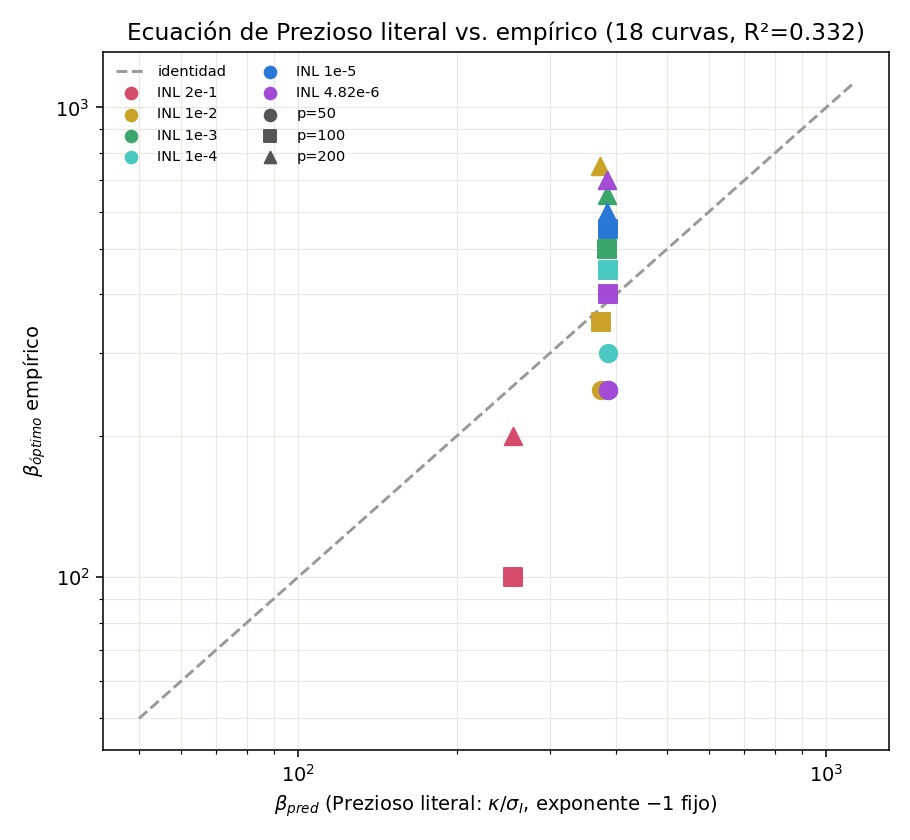
\includegraphics[width=0.72\linewidth]{prezioso_literal_vs_empirico.png}
\caption{Ecuación de Prezioso literal (exponente $-1$ fijo, $\sigma_I$ del MC corregido) vs.\ $\beta$ óptimo empírico.}
\end{figure}

La figura lo muestra claramente: como $\sigma_W$ (MC corregido) apenas
varía entre curvas de igual INL nominal pero distinto $p$ (el INL nominal
domina, no la cantidad de pulsos), la ecuación con exponente $-1$
\textbf{predice casi el mismo $\beta$ para las 3 curvas de un mismo INL},
sin importar que el $\beta$ óptimo real varíe hasta $3\times$ entre ellas
($p=50$ vs.\ $p=200$). \textbf{Conclusión: la ecuación de Prezioso, tal
como está citada (exponente $-1$), NO calcula bien el $\beta$ óptimo
experimental de estas 18 curvas} --- confirma y extiende (ahora con 18
puntos en vez de 6, y con datos reales reconstruidos en vez de solo
sintéticos) lo ya encontrado en \texttt{validacion\_formula\_beta\_optimo/}.

\section{Resultado 3: la ecuación mejorada -- y por qué no conviene usar $\sigma_I$ real}

Siguiendo el pedido ("estudia la data para obtener una ecuación que dé un
mejor resultado"), se repitieron las regresiones log-log de
\texttt{formula\_beta\_optimo\_propuesta\_v2} pero probando además las 2
fuentes NUEVAS de $\sigma_I$ (reales, de esta sesión) en vez de/además del
MC corregido:

\begin{figure}[htbp]
\centering
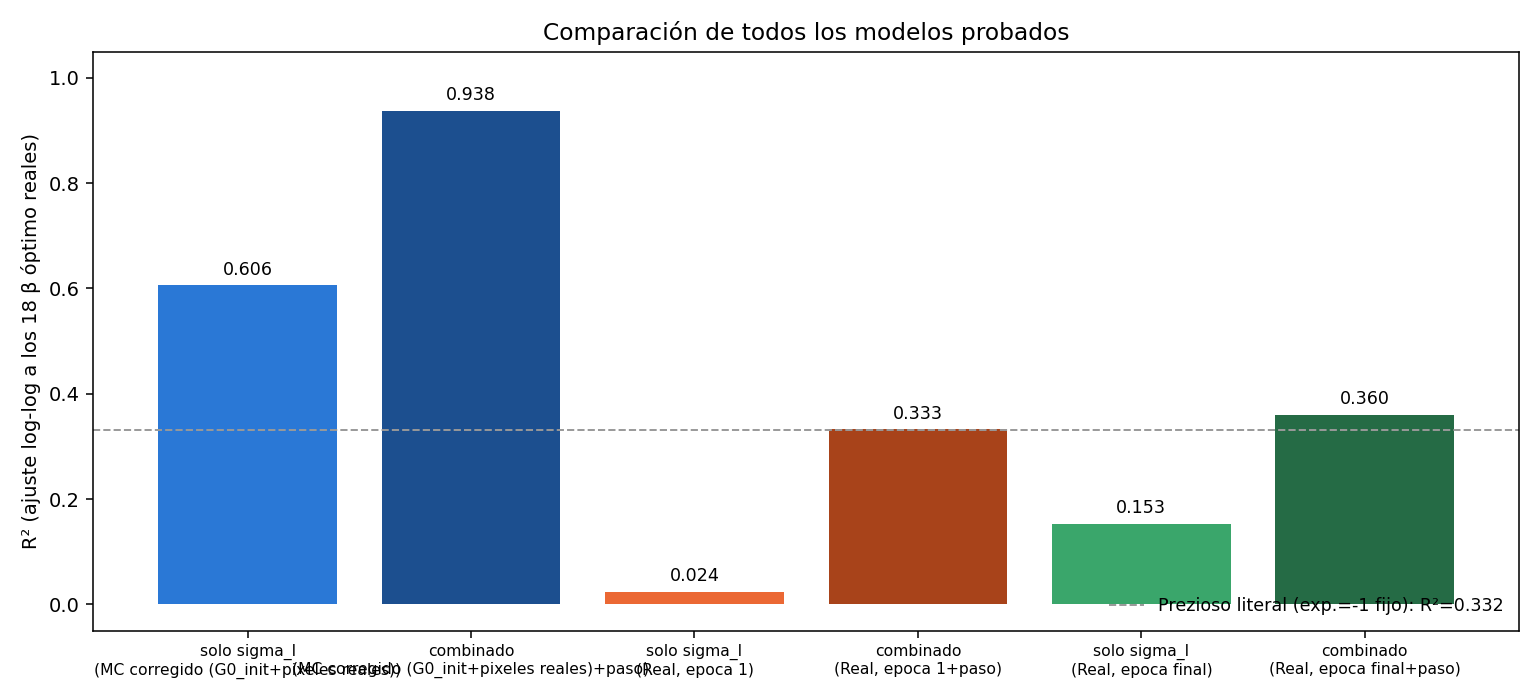
\includegraphics[width=\linewidth]{comparacion_R2_todos_los_modelos.png}
\caption{$R^2$ de los 6 modelos probados (18 curvas). Línea gris: Prezioso literal.}
\end{figure}

\begin{table}[htbp]
\centering
\begin{tabular}{@{}lr@{}}
\toprule
Modelo & $R^2$ \\
\midrule
solo $\sigma_I$ (MC corregido) & 0.606 \\
\textbf{combinado ($\sigma_I$ MC corregido + paso\_medio)} & \textbf{0.938} \\
solo $\sigma_I$ (real, época 1) & 0.024 \\
combinado ($\sigma_I$ real época 1 + paso\_medio) & 0.333 \\
solo $\sigma_I$ (real, época final) & 0.153 \\
combinado ($\sigma_I$ real época final + paso\_medio) & 0.360 \\
\bottomrule
\end{tabular}
\end{table}

\textbf{Usar la corriente REAL reconstruida en vez del MC corregido no
mejora la ecuación -- la empeora drásticamente} (0.938 $\to$ 0.33--0.36).
La razón es exactamente la de la Sección~3: $\sigma_I$ real varía muy poco
entre curvas (todas convergen cerca de 0.031--0.032), así que casi no
aporta información -- los modelos "combinados" con $\sigma_I$ real quedan
reducidos, en la práctica, a depender solo de \texttt{paso\_medio}
(compárese 0.333 y 0.360 aquí con el 0.333 de "solo paso\_medio" en
\texttt{formula\_beta\_optimo\_propuesta\_v2}). El coeficiente ajustado de
$\log(\sigma_I\text{ real época 1})$ en el modelo combinado es
$+0.011$ -- prácticamente cero.

\textbf{La ecuación mejorada sigue siendo, entonces, la ya derivada en
\texttt{formula\_beta\_optimo\_propuesta\_v2.py}} (ahora reconfirmada:
mismos coeficientes, mismo $R^2=0.938$, sobre las mismas 18 curvas, con el
extra de haber probado explícitamente que agregar la corriente real
reconstruida no ayuda):
\begin{equation}
\beta_{\text{óptimo}} \;\approx\; 1.34\times10^{-11}\cdot\sigma_W^{-3.05}\cdot\mathrm{paso\_medio}^{-0.61}
\label{eq:combinada}
\end{equation}
donde $\sigma_W$ es el del MC corregido (inicialización real, antes de
entrenar) y \texttt{paso\_medio} $=\mathrm{mean}(|\mathrm{pot}[i{+}1]-\mathrm{pot}[i]|)$.

\begin{figure}[htbp]
\centering
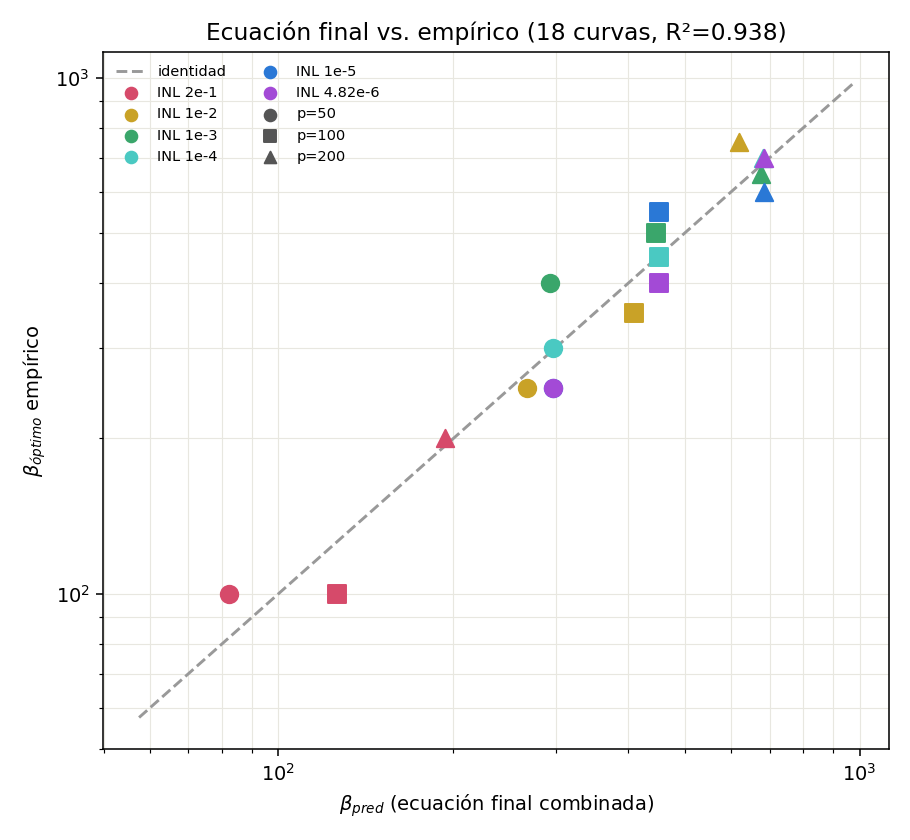
\includegraphics[width=0.68\linewidth]{ecuacion_final_vs_empirico.png}
\caption{Ecuación mejorada (Ec.~\ref{eq:combinada}) vs.\ $\beta$ óptimo empírico, 18 curvas.}
\end{figure}

\section{Recomendaciones y datos adicionales necesarios}

\begin{itemize}
\item \textbf{Zona de transición INL (entre 2e-1 y 1e-2).} Casi toda la
  variación de forma de la curva P/D (y, en menor medida, del
  aplanamiento de accuracy-vs-beta) ocurre en esa única década; hoy solo
  hay 2 puntos ahí. Los INL=5e-2/5e-3/5e-4/5e-5 recién corridos ayudan;
  agregar 1e-1 completaría mejor esa zona.
\item \textbf{Tamaño de crossbar $N$.} Las 18 curvas comparten $N=784$
  (fan-in de MNIST): el exponente de $N$ en la Ec.~\ref{eq:prezioso}
  ($N^{-1/2}$) sigue sin poder testearse con esta data; el reporte
  analítico previo encontró $\sim N^{-1.05}$ con una búsqueda reducida (1
  época) -- confirmar con entrenamiento completo es la mejora de mayor
  impacto pendiente.
\item \textbf{Otro dataset (Fashion-MNIST ya disponible).} Probaría si
  $V_{\mathrm{rms}}$ realmente importa, sin generar curvas P/D nuevas.
\item \textbf{Grilla de $\beta$ más fina cerca del óptimo.} El $\beta$
  óptimo actual sale de una grilla de 40 puntos espaciados de a 50; una
  segunda pasada más fina reduciría el ruido de la variable que se está
  intentando predecir.
\end{itemize}

\section{Análisis crítico: ¿Monte Carlo de un solo paso, o seguir con \texttt{search\_best\_beta()}?}

La Ec.~\ref{eq:combinada} predice el $\beta$ óptimo real con error entre
$-27\%$ y $+26\%$ (escala log) sobre las 18 curvas -- no es exacta. La
pregunta es si ese error es lo bastante chico como para no necesitar
ninguna búsqueda, o si conviene seguir usando \texttt{search\_best\_beta()}.

\textbf{Chequeo concreto:} para cada una de las 18 curvas, se comparó el
$\beta$ predicho por la Ec.~\ref{eq:combinada} contra el ancho de la
meseta empírica al 99\% del pico de accuracy (de
\texttt{formula\_beta\_optimo\_propuesta\_v2/resultados\_formula\_propuesta\_v2.csv},
aproximando esa meseta como simétrica alrededor del $\beta$ óptimo real).
Resultado: \textbf{en las 18 de 18 curvas, el $\beta$ predicho cae DENTRO
de esa meseta} -- es decir, entrenar con el $\beta$ que predice la
ecuación (sin ninguna búsqueda) habría dado, en los 18 casos probados,
$\geq99\%$ de la mejor accuracy alcanzable en esa curva.

Esto es alentador, pero hay 3 razones para no confiar en la ecuación como
reemplazo total de \texttt{search\_best\_beta()}:
\begin{enumerate}
\item El criterio "99\% del pico" es una aproximación (meseta simétrica,
  grilla de 40 puntos de por sí gruesa) -- no es una garantía formal.
\item La muestra sigue siendo chica y con $N$/dataset fijos (Sección~6):
  el error real fuera de este régimen exacto (SP, $N=784$, MNIST) es
  desconocido.
\item El hallazgo de la Sección~3 (la corriente REAL converge a un valor
  casi universal, sin importar la curva P/D) sugiere algo más profundo:
  \textbf{cualquier estimador que solo mire la curva P/D "antes de
  entrenar" tiene un techo de precisión inherente}, porque el propio
  entrenamiento reorganiza la red hacia una escala de corriente que
  depende del dataset/arquitectura/optimización, no solo de la curva P/D.
  La Ec.~\ref{eq:combinada} funciona razonablemente bien (R²=0.94) PRECISAMENTE
  porque usa $\sigma_W$ de inicialización (lo único disponible sin
  entrenar) -- pero no hay forma de que un método de un solo paso, sin
  entrenar nada, capture con precisión perfecta cómo el entrenamiento va a
  reorganizar esa corriente.
\end{enumerate}

\textbf{Recomendación:} no reemplazar \texttt{search\_best\_beta()} por la
Ec.~\ref{eq:combinada} en modo "un solo paso, sin verificar". En cambio,
usarla como \textbf{pre-filtro}: calcular $\beta_{\text{pred}}$ con la
Ec.~\ref{eq:combinada} (barato, sin entrenar nada) y correr
\texttt{search\_best\_beta()} en una ventana ANGOSTA alrededor de ese valor
(p.ej.\ $\beta_{\text{pred}}\times[0.5, 2]$ con 5--7 puntos) en vez de la
grilla completa actual (1--1950, 40 puntos) -- un ahorro de cómputo de
$\sim5$--$8\times$ sin perder la garantía de una búsqueda real. Cuando el
costo de entrenar sea tan alto que ni una búsqueda angosta sea viable, la
evidencia de este reporte (18/18 dentro de la meseta al 99\%) sugiere que
usar $\beta_{\text{pred}}$ directamente es una apuesta razonable -- pero
debe entenderse como eso, una apuesta respaldada por 18 ejemplos en un
único régimen, no una garantía.

\section{Conclusión}

\begin{enumerate}
\item Los logits/corrientes de validación se reconstruyeron EXACTO
  (sanity check sin ninguna discrepancia) para las 18 curvas, en función
  de la época, sin reentrenar nada.
\item La corriente real converge, en menos de 10 épocas, a un valor de
  $\sigma_I$ casi universal ($\approx0.031$--$0.032$) sin importar INL ni
  pulsos -- 5--9$\times$ por encima de cualquiera de los dos Monte Carlo.
\item La ecuación de Prezioso literal (exponente $-1$ fijo) NO explica el
  $\beta$ óptimo de estas 18 curvas ($R^2$ entre $-0.07$ y $0.33$ según la
  fuente de $\sigma_I$).
\item La ecuación mejorada ya derivada
  ($\beta_{\text{óptimo}}\approx1.34\times10^{-11}\sigma_W^{-3.05}\mathrm{paso\_medio}^{-0.61}$,
  $R^2=0.938$) se reconfirma como la mejor disponible -- y se confirma que
  usar la corriente REAL reconstruida en vez del $\sigma_W$ de
  inicialización no la mejora (la empeora), por una razón mecanicista
  clara (Sección~3).
\item Un Monte Carlo de un solo paso (la Ec.~\ref{eq:combinada}) es útil
  como \textbf{pre-filtro barato} para acotar el rango de
  \texttt{search\_best\_beta()}, no como reemplazo total: en los 18 casos
  probados habría bastado solo, pero la muestra y el argumento mecanicista
  de la Sección~3 recomiendan mantener una verificación angosta.
\end{enumerate}

\section{Registro de códigos usados}

\begin{itemize}
\item \textbf{\texttt{reconstruir\_corrientes\_18curvas.py}} --- reconstruye
  logits/corrientes reales (18 curvas, $\beta=1$, serie 0) y calcula los 2
  Monte Carlo de referencia. Genera \texttt{resultados\_18curvas.csv},
  \texttt{trayectorias\_std\_18curvas.png}, \texttt{comparacion\_sigma\_fuentes.png}.
\item \textbf{\texttt{probar\_prezioso\_y\_regresiones.py}} --- prueba la
  Ec.~\ref{eq:prezioso} literal y ajusta las 6 regresiones log-log. Genera
  \texttt{resultados\_prezioso.csv}, \texttt{coeficientes\_todos\_los\_modelos.csv}
  y las 3 figuras de comparación.
\item \texttt{reconstruccion\_logits\_val\_INL\_1e-2\_p\_100\_beta1/reconstruir\_logits\_val.py} ---
  ejemplo detallado (1 curva) con el sanity check exacto documentado.
\item \texttt{formula\_beta\_optimo\_propuesta/estimar\_beta\_optimo\_propuesta\_v2.py} ---
  origen de la Ec.~\ref{eq:combinada} y de \texttt{paso\_medio}/\texttt{ancho99}.
\item \texttt{MemCrossbarClass\_beta\_por\_capa.py} $\to$
  \texttt{generar\_curvas\_pot\_dep()}, \texttt{G0\_initialization()} ---
  usadas sin modificar.
\item \texttt{analisis\_beta\_optimo.py} --- MC sesgado, usado sin modificar
  como referencia.
\item \texttt{papers/Reporte\_beta\_optimo\_analitico.pdf} --- origen de la
  Ec.~\ref{eq:prezioso} y de \texttt{paso\_medio}.
\item \texttt{data\_beta\_grid\_search\_SP/beta\_grid\_search\_SP\_INL\_*/}
  (config, resultados, G\_history) --- las 18 corridas reales usadas.
\end{itemize}

Archivos generados por este reporte (todos en
\texttt{reconstruccion\_beta\_optimo\_18curvas/}):
\texttt{reconstruir\_corrientes\_18curvas.py},
\texttt{probar\_prezioso\_y\_regresiones.py},
\texttt{resultados\_18curvas.csv}, \texttt{resultados\_prezioso.csv},
\texttt{coeficientes\_todos\_los\_modelos.csv},
\texttt{trayectorias\_std\_18curvas.png}, \texttt{comparacion\_sigma\_fuentes.png},
\texttt{prezioso\_literal\_vs\_empirico.png},
\texttt{comparacion\_R2\_todos\_los\_modelos.png},
\texttt{ecuacion\_final\_vs\_empirico.png},
\texttt{reporte\_reconstruccion\_beta\_optimo.tex} y este PDF.

\end{document}
